\documentclass[aspectratio=169]{beamer}
\mode<presentation>

\usepackage{graphicx}

\usepackage{tikz}
\usetikzlibrary{arrows.meta}
\usetikzlibrary{fit}
\usetikzlibrary{positioning}
\usetikzlibrary{shapes.multipart}
\usetikzlibrary{shadows}
\usetikzlibrary{tikzmark}

\title{Stack Graphs}
\author{Douglas Creager}
\institute{GitHub}
\date{Strange Loop 2021}

\setbeamertemplate{navigation symbols}{}

\usepackage{minted}
\usemintedstyle{colorful}

\usepackage{fontspec}
\setsansfont{Arial}
\setmonofont[Scale=0.8]{Iosevka Term}

\newlength{\scopegap}
\setlength{\scopegap}{0.9cm}

\definecolor{sgdef}  {RGB}{159,0,0}
\definecolor{sgpop}  {RGB}{230,142,131}
\definecolor{sgref}  {RGB}{0,134,67}
\definecolor{sgpush} {RGB}{131,216,173}
\definecolor{sgjump} {RGB}{161,64,140}

\tikzset{root node/.style={
    node distance=0.5cm,
    circle, fill=black, inner sep=0pt,
    minimum size=0.35cm
}}

\tikzset{anon scope/.style={
    node distance=0.5cm,
    circle, fill=white, inner sep=0pt,
    draw=black, semithick,
    minimum size=0.35cm
}}

\tikzset{named scope/.style={
    node distance=0.5cm,
    circle, fill=white,
    draw=black, thick,
    minimum size=0.35cm
}}

\tikzset{exported scope/.style={
    node distance=0.5cm,
    circle, fill=white,
    draw=sgjump, thick, text=sgjump,
    minimum size=0.35cm
}}

\tikzset{symbol text/.style={
    fill=white,
    text height=1.5ex, text depth=0.25ex, node font=\ttfamily,
    inner xsep=7pt,
    minimum size=0.75cm,
}}

\tikzset{definition/.style={
    node distance=0.5cm,
    draw=sgdef, semithick, double, double distance=1pt, outer sep=1pt,
    text=sgdef, symbol text,
}}

\tikzset{pop/.style={
    node distance=0.5cm,
    rectangle split,
    rectangle split parts=2,
    rectangle split horizontal,
    rectangle split draw splits=false,
    rectangle split ignore empty parts,
    draw=sgpop, thick, dash dot,
    text=sgpop, symbol text,
}}
\newcommand{\popscope}{
    \nodepart{two}
    \hspace{-12pt}
    \tikz \node [circle, fill=sgjump, inner sep=0pt, minimum size=0.25cm] {};
}

\tikzset{reference/.style={
    node distance=0.5cm,
    draw=sgref, thick,
    text=sgref, symbol text,
}}

\tikzset{push/.style={
    node distance=0.5cm,
    rectangle split,
    rectangle split parts=2,
    rectangle split horizontal,
    rectangle split draw splits=false,
    rectangle split ignore empty parts,
    draw=sgpush, thick, densely dashed,
    text=sgpush, symbol text,
}}
\newcommand{\pushscope}[1]{
    \nodepart{two}
    \hspace{-12pt}
    \tikz \node [
        circle, fill=white,
        draw=sgjump,
        text=sgjump, inner sep=2pt,
        minimum size=0.25cm
    ] {\tiny #1};
}

\newcommand{\widestsymbol}{}
\newcommand{\setwidestsymbol}[1]{\renewcommand{\widestsymbol}{#1}}
\newcommand{\sized}[2][\widestsymbol]{\makebox[\widthof{#1}]{#2}}

\tikzset{
  alt/.code args={<#1>#2#3}{%
    \alt<#1>{\pgfkeysalso{#2}}{\pgfkeysalso{#3}} % \pgfkeysalso doesn't change the path
  }
}

\tikzset{
    highlight node/.style={
        general shadow={fill=blue, opacity=0.3},
        shadow scale=1.2, shadow xshift=0pt, shadow yshift=0pt
    }
}
\tikzset{
    highlight node on/.code args={<#1>}{%
        \alt<#1>{\pgfkeysalso{highlight node}}{}%
    }
}

% Animating paths in a stack graph picture
%   Just add [highlighted on=<slide>] to an edge's style.  The line of the edge
%   will be blue and extra thick on <slide> AND ALL LATER SLIDES.  It will have
%   an arrowhead on SLIDE.
%
%   Together, this means that you add this to all of the edges that comprise a
%   path, with increasing <slide> values for each one, and beamer will create an
%   overlay animation showing the edges of the path get highlighted in order
%   each time you advance to the next slide.
\tikzset{highlight edge/.style={line width=2pt, blue, -}}
\tikzset{highlight edge frontier/.style={-{Triangle[length=4pt,width=4pt]}}}
\tikzset{
    show path on/.code args={<#1>}{%
        \alt<#1- >{\pgfkeysalso{highlight edge}}{}%
        \alt<#1  >{\pgfkeysalso{highlight edge frontier}}{}%
    }
}

\tikzset{binding arrow/.style={->, red, thick, -{Triangle[]}}}

\newcommand{\codeline}[3][]{%
    \tikz[remember picture] \draw [overlay, binding arrow, #1] (#2) -- (#3);%
}

\newcommand{\curvecodeline}[4][]{%
    \tikz[remember picture] \draw [overlay, binding arrow, #1] (#2) .. controls #3 .. (#4);%
}

\newcommand{\highlightdef}[1]{%
    \tikz[remember picture]
      \draw [overlay, draw=none, fill=red!25]
        ([xshift=-1pt, yshift=8pt] pic cs:#1_start)
        rectangle
        ([xshift=1pt, yshift=-2pt] pic cs:#1_end)
        ;
}

\newcommand{\highlightref}[1]{%
    \tikz[remember picture]
      \draw [overlay, draw=none, fill=blue!25]
        ([xshift=-1pt, yshift=8pt] pic cs:#1_start)
        rectangle
        ([xshift=1pt, yshift=-2pt] pic cs:#1_end)
        ;
}


\begin{document}

\begin{frame}
    \titlepage
\end{frame}


\section{Code Navigation}

\begin{frame}
    \sectionpage
\end{frame}

% easy
\begin{frame}[fragile]
    \frametitle{Code Navigation}
    \begin{center}
    \begin{minipage}{9em}
    \begin{minted}[autogobble,frame=single,framesep=6pt,label=stove.py,escapeinside=??]{python}
        def bake():
            pass

        def broil?\tikzmark{easy_broil_def}?():
            pass

        def saute():
            pass

        broil?\tikzmark{easy_broil_ref}?()
    \end{minted}
    \end{minipage}
    \end{center}
    \uncover<2>{\curvecodeline%
      {[yshift=8pt] pic cs:easy_broil_ref}%
      {+(25:2cm) and +(-45:1cm)}%
      {[yshift=-4pt] pic cs:easy_broil_def}%
    }%
\end{frame}


\section{Why is this hard?}

\begin{frame}
    \sectionpage
\end{frame}


% easy_shadowed
\begin{frame}[fragile]
    \frametitle{Why is this hard?}
    \begin{center}
    \begin{minipage}{9em}
    \begin{minted}[autogobble,frame=single,framesep=6pt,label=stove.py,escapeinside=??]{python}
        def broil?\tikzmark{easy_shadowed_broil_def1}?():
            pass

        def broil?\tikzmark{easy_shadowed_broil_def2}?():
            pass

        def saute():
            pass

        broil?\tikzmark{easy_shadowed_broil_ref}?()
    \end{minted}
    \end{minipage}
    \end{center}
    \uncover<2>{\curvecodeline%
      [dotted]%
      {[yshift=8pt] pic cs:easy_shadowed_broil_ref}%
      {+(15:3cm) and +(-35:1cm)}%
      {[yshift=-4pt] pic cs:easy_shadowed_broil_def1}%
    }%
    \uncover<2>{\curvecodeline%
      {[yshift=8pt] pic cs:easy_shadowed_broil_ref}%
      {+(25:2cm) and +(-45:1cm)}%
      {[yshift=-4pt] pic cs:easy_shadowed_broil_def2}%
    }%
\end{frame}


% easy_shadowed_rust
\begin{frame}[fragile]
    \frametitle{Why is this hard?}
    \begin{center}
    \begin{minipage}{9em}
    \begin{minted}[autogobble,frame=single,framesep=6pt,label=stove.rs,escapeinside=??]{rust}
        fn broil() {}

        fn broil?\tikzmark{easy_shadowed_rust_broil_def2}?() {}

        fn saute() {}

        fn main() {
          broil();
        }
    \end{minted}
    \end{minipage}
    \end{center}
    \uncover<2>{%
        \tikz[remember picture]
          \node [overlay, text=red]
            at ([xshift=-2ex, yshift=0.5ex] pic cs:easy_shadowed_rust_broil_def2)
            {\textbf{\Huge X}};%
    }%
\end{frame}


% separate_files
\begin{frame}[fragile]
    \frametitle{Why is this hard?}
    \begin{center}
    \begin{minipage}[t]{9em}
    \begin{minted}[autogobble,frame=single,framesep=6pt,label=stove.py,escapeinside=??]{python}
        def bake():
            pass

        def broil?\tikzmark{separate_files_broil_def}?():
            pass

        def saute():
            pass
    \end{minted}
    \end{minipage}
    \hspace{0.5em}
    \begin{minipage}[t]{11em}
    \begin{minted}[autogobble,frame=single,framesep=6pt,label=kitchen.py,escapeinside=??]{python}
        from stove import ?\tikzmark{separate_files_broil_import}?broil

        broil?\tikzmark{separate_files_broil_ref}?()
    \end{minted}
    \end{minipage}
    \end{center}
    \uncover<2>{\curvecodeline%
      [-]%
      {[yshift=10pt] pic cs:separate_files_broil_ref}%
      {+(45:1cm) and +(-155:1cm)}%
      {[yshift=-4pt] pic cs:separate_files_broil_import}%
    }
    \uncover<2>{\curvecodeline%
      {[xshift=12pt, yshift=10pt] pic cs:separate_files_broil_import}%
      {+(90:2cm) and +(75:2cm)}%
      {[xshift=-6pt, yshift=10pt] pic cs:separate_files_broil_def}%
    }
\end{frame}


% separate_files_star
\begin{frame}[fragile]
    \frametitle{Why is this hard?}
    \begin{center}
    \begin{minipage}[t]{9em}
    \begin{minted}[autogobble,frame=single,framesep=6pt,label=stove.py,escapeinside=??]{python}
        def bake():
            pass

        def broil?\tikzmark{separate_files_star_broil_def}?():
            pass

        def saute():
            pass
    \end{minted}
    \end{minipage}
    \hspace{0.5em}
    \begin{minipage}[t]{11em}
    \begin{minted}[autogobble,frame=single,framesep=6pt,label=kitchen.py,escapeinside=??]{python}
        from stove import ?\tikzmark{separate_files_star_import}?*

        broil?\tikzmark{separate_files_star_broil_ref}?()
    \end{minted}
    \end{minipage}
    \end{center}
    \uncover<2>{\curvecodeline%
      [-]%
      {[yshift=10pt] pic cs:separate_files_star_broil_ref}%
      {+(45:1cm) and +(-105:1cm)}%
      {[xshift=1pt, yshift=-2pt] pic cs:separate_files_star_import}%
    }
    \uncover<2>{\curvecodeline%
      {[xshift=3pt, yshift=10pt] pic cs:separate_files_star_import}%
      {+(90:2cm) and +(75:2cm)}%
      {[xshift=-6pt, yshift=10pt] pic cs:separate_files_star_broil_def}%
    }
\end{frame}


% three_files
\begin{frame}[fragile]
    \frametitle{Why is this hard?}
    \begin{center}
    \begin{minipage}[t]{22.5em}
    \begin{center}
        
\includegraphics[height=2em]{images/pan.png}
    \end{center}
    \vskip -1em
    \begin{minipage}[t]{7em}
    \begin{minted}[autogobble,frame=single,framesep=6pt,label=stove.py,escapeinside=??]{python}
        def bake():
            pass

        def broil?\tikzmark{three_files_broil_def}?():
            pass

        def saute():
            pass
    \end{minted}
    \end{minipage}
    \hspace{0.5em}
    \begin{minipage}[t]{15em}
    \begin{minted}[autogobble,frame=single,framesep=6pt,label=kitchen.py,escapeinside=??]{python}
        from stove import ?\tikzmark{three_files_kitchen_import}?*
    \end{minted}
    \end{minipage}
    \end{minipage}
    \hspace{0.5em}
    \begin{minipage}[t]{12em}
    \vskip 8em
    \begin{center}
        
\includegraphics[height=2em]{images/chef.png}
    \end{center}
    \begin{minted}[autogobble,frame=single,framesep=6pt,label=chef.py,escapeinside=??]{python}
        from kitchen import ?\tikzmark{three_files_chef_import}?broil

        broil?\tikzmark{three_files_broil_ref}?()
    \end{minted}
    \end{minipage}
    \end{center}
    \uncover<2>{\curvecodeline%
      [-]%
      {[yshift=10pt] pic cs:three_files_broil_ref}%
      {+(45:1cm) and +(-155:1cm)}%
      {[yshift=-4pt] pic cs:three_files_chef_import}%
    }
    \uncover<2>{\curvecodeline%
      [-]%
      {[xshift=10pt, yshift=10pt] pic cs:three_files_chef_import}%
      {+(90:5cm) and +(75:2cm)}%
      {[xshift=4pt, yshift=10pt] pic cs:three_files_kitchen_import}%
    }
    \uncover<2>{\curvecodeline%
      {[xshift=1pt, yshift=-4pt] pic cs:three_files_kitchen_import}%
      {+(-105:1cm) and +(75:1cm)}%
      {[xshift=-6pt, yshift=10pt] pic cs:three_files_broil_def}%
    }
\end{frame}


% three_files_updated
\begin{frame}[fragile]
    \frametitle{Why is this hard?}
    \begin{center}
    \begin{minipage}[t]{22.5em}
    \begin{center}
        
\includegraphics[height=2em]{images/pan.png}
    \end{center}
    \vskip -1em
    \begin{minipage}[t]{7em}
    \begin{minted}[autogobble,frame=single,framesep=6pt,label=stove.py,escapeinside=??]{python}
        def bake():
            pass

        def broil():
            pass

        def saute():
            pass
    \end{minted}
    \end{minipage}
    \hspace{0.5em}
    \begin{minipage}[t]{15em}
    \begin{minted}[autogobble,frame=single,framesep=6pt,label=kitchen.py,escapeinside=??]{python}
        from stove import *

        def broil?\tikzmark{three_files_updated_broil_def}?():
            print("We're broiling!")
            import stove
            return stove.broil()
    \end{minted}
    \end{minipage}
    \end{minipage}
    \hspace{0.5em}
    \begin{minipage}[t]{12em}
    \vskip 8em
    \begin{center}
        
\includegraphics[height=2em]{images/chef.png}
    \end{center}
    \begin{minted}[autogobble,frame=single,framesep=6pt,label=chef.py,escapeinside=??]{python}
        from kitchen import ?\tikzmark{three_files_updated_chef_import}?broil

        broil?\tikzmark{three_files_updated_broil_ref}?()
    \end{minted}
    \end{minipage}
    \end{center}
    \uncover<2>{\curvecodeline%
      [-]%
      {[yshift=10pt] pic cs:three_files_updated_broil_ref}%
      {+(45:1cm) and +(-155:1cm)}%
      {[yshift=-4pt] pic cs:three_files_updated_chef_import}%
    }
    \uncover<2>{\curvecodeline%
      {[xshift=10pt, yshift=10pt] pic cs:three_files_updated_chef_import}%
      {+(90:5cm) and +(75:2cm)}%
      {[xshift=-6pt, yshift=10pt] pic cs:three_files_updated_broil_def}%
    }
\end{frame}


% python_class
\begin{frame}[fragile]
    \frametitle{Why is this hard?}
    \begin{center}
    \begin{minipage}[t]{25.5em}
    \begin{center}
        
\includegraphics[height=2em]{images/pan.png}
    \end{center}
    \vskip -1em
    \begin{minipage}[t]{10em}
    \begin{minted}[autogobble,frame=single,framesep=6pt,label=stove.py,escapeinside=??]{python}
        class?\tikzmark{python_class_stove_class}? Stove?\tikzmark{python_class_stove_class_def}?(object):
            def bake():
                pass

            def broil?\tikzmark{python_class_broil_def}?():
                pass

            def saute():
                pass
    \end{minted}
    \end{minipage}
    \hspace{0.5em}
    \begin{minipage}[t]{15em}
    \begin{minted}[autogobble,frame=single,framesep=6pt,label=kitchen.py,escapeinside=??]{python}
        from stove import ?\tikzmark{python_class_kitchen_import}?*
    \end{minted}
    \end{minipage}
    \end{minipage}
    \hspace{-5.5em}
    \begin{minipage}[t]{12em}
    \vskip 6em
    \begin{center}
        
\includegraphics[height=2em]{images/chef.png}
    \end{center}
    \begin{minted}[autogobble,frame=single,framesep=6pt,label=chef.py,escapeinside=??]{python}
        from kitchen import ?\tikzmark{python_class_chef_import}?Stove

        stove?\tikzmark{python_class_stove_instance_def}? = Stove?\tikzmark{python_class_stove_class_ref}?()
        stove?\tikzmark{python_class_stove_instance_ref}?.broil?\tikzmark{python_class_broil_ref}?()
    \end{minted}
    \end{minipage}
    \end{center}
    \uncover<2- >{\curvecodeline%
      [-, alt=<3>{line width=2pt, blue}{}]%
      {[xshift=-10pt, yshift=-3pt] pic cs:python_class_broil_ref}%
      {+(-135:0.2cm) and +(-45:0.2cm)}%
      {[xshift=-10pt, yshift=-3pt] pic cs:python_class_stove_instance_ref}%
    }
    \uncover<2- >{\curvecodeline%
      [-, alt=<4>{line width=2pt, blue}{}]%
      {[xshift=-23pt, yshift=2pt] pic cs:python_class_stove_instance_ref}%
      {+(180:0.2cm) and +(180:0.2cm)}%
      {[xshift=-23pt, yshift=2pt] pic cs:python_class_stove_instance_def}%
    }
    \uncover<2- >{\curvecodeline%
      [-, alt=<5>{line width=2pt, blue}{}]%
      {[xshift=-10pt, yshift=8pt] pic cs:python_class_stove_instance_def}%
      {+(65:0.3cm) and +(115:0.3cm)}%
      {[xshift=-10pt, yshift=8pt] pic cs:python_class_stove_class_ref}%
    }
    \uncover<2- >{\curvecodeline%
      [-, alt=<6>{line width=2pt, blue}{}]%
      {[xshift=-4pt, yshift=-3pt] pic cs:python_class_stove_class_ref}%
      {+(-35:0.5cm) and +(-90:1cm)}%
      {[xshift=10pt, yshift=-3pt] pic cs:python_class_chef_import}%
    }
    \uncover<2- >{\curvecodeline%
      [-, alt=<7>{line width=2pt, blue}{}]%
      {[xshift=10pt, yshift=10pt] pic cs:python_class_chef_import}%
      {+(90:3cm) and +(-90:1cm)}%
      {[xshift=2pt, yshift=-3pt] pic cs:python_class_kitchen_import}%
    }
    \uncover<2- >{\curvecodeline%
      [-, alt=<8>{line width=2pt, blue}{}]%
      {[xshift=2pt, yshift=10pt] pic cs:python_class_kitchen_import}%
      {+(90:2cm) and +(90:2cm)}%
      {[xshift=-10pt, yshift=8pt] pic cs:python_class_stove_class_def}%
    }
    \uncover<2- >{\curvecodeline%
      [-, alt=<9>{line width=2pt, blue}{}]%
      {[xshift=-6pt, yshift=-2pt] pic cs:python_class_stove_class_def}%
      {+(-45:2cm) and +(90:2cm)}%
      {[xshift=4pt, yshift=10pt] pic cs:python_class_stove_class_ref}%
    }
    \uncover<2- >{\curvecodeline%
      [-, alt=<10>{line width=2pt, blue}{}]%
      {[xshift=4pt, yshift=-3pt] pic cs:python_class_stove_class_ref}%
      {+(-90:2.5cm) and +(-90:6.5cm)}%
      {[xshift=-10pt, yshift=-2pt] pic cs:python_class_stove_class}%
    }
    \uncover<2- >{\curvecodeline%
      [alt=<11>{line width=2pt, blue}{}]%
      {[xshift=-10pt, yshift=8pt] pic cs:python_class_stove_class}%
      {+(75:1cm) and +(115:1cm)}%
      {[xshift=-10pt, yshift=6pt] pic cs:python_class_broil_def}%
    }
\end{frame}


\begin{frame}
    \frametitle{Zero configuration}
    \begin{center}
        We don't want to have to ask the package \\ owner how to collect the data
        we need.
    \end{center}
    \begin{center}
        Or ask them to configure a job to produce that data.
    \end{center}
    \begin{center}
        We \strong{especially} can't ask an open-source maintainer \\ to expend
        effort to generate data that we need \\ for an enterprise customer!
    \end{center}
\end{frame}


\begin{frame}
    \frametitle{SCALE}
    \emph{Quote some big numbers about GitHub's scale}
\end{frame}


\begin{frame}
    \frametitle{Incremental processing}
    \begin{center}
        In a typical commit, a small fraction of files in the repo change.
    \end{center}
    \begin{center}
        We want to reuse results that we've \\ already calculated for unchanged
        files.
    \end{center}
    \begin{center}
        \emph{Structural sharing} (like git itself) helps save storage.
    \end{center}
    \begin{center}
        \emph{Incremental processing} also helps save compute.
    \end{center}
\end{frame}


\begin{frame}
    \frametitle{Why is this hard?}
    \begin{itemize}
        \item Different languages have different name binding rules.
        \item Some of those rules can be quite complex.
        \item The result might depend on intermediate files.
        \item We don't want to require manual per-repo configuration.
        \item We need incremental processing to handle our scale.
    \end{itemize}
\end{frame}


\begin{frame}[t]
    \frametitle{When do we do the work?}
    \vskip 2em
    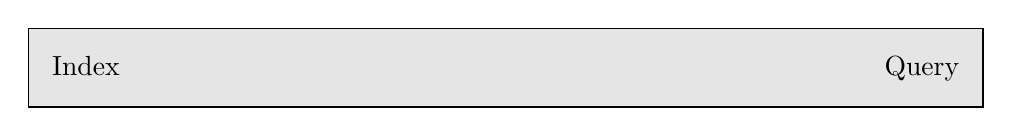
\begin{tikzpicture}
        \node (bar) at(0,0) [
            rectangle, anchor=west,
            minimum width=\columnwidth, minimum height=1cm,
            draw=black, thin,
            fill=gray!20,
        ] {};

        \node at(bar.west) [
            rectangle, anchor=west, inner xsep=2ex,
            text height=1.5ex, text depth=0.25ex,
            text=black,
        ] {Index};
        \node at(bar.east) [
            rectangle, anchor=east, inner xsep=2ex,
            text height=1.5ex, text depth=0.25ex,
            text=black,
        ] {Query};
    \end{tikzpicture}
\end{frame}


\begin{frame}[t]
    \frametitle{When do we do the work?}
    \vskip 2em
    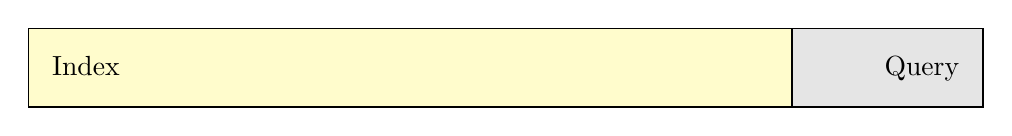
\begin{tikzpicture}
        \node (bar) at(0,0) [
            rectangle, anchor=west,
            minimum width=\columnwidth, minimum height=1cm,
            draw=black, thin,
            fill=gray!20,
        ] {};

        \node at(bar.west) [
            rectangle, anchor=west,
            minimum width=0.8\columnwidth, minimum height=1cm,
            draw=black, thin,
            fill=yellow!20,
        ] {};

        \node at(bar.west) [
            rectangle, anchor=west, inner xsep=2ex,
            text height=1.5ex, text depth=0.25ex,
            text=black,
        ] {Index};
        \node at(bar.east) [
            rectangle, anchor=east, inner xsep=2ex,
            text height=1.5ex, text depth=0.25ex,
            text=black,
        ] {Query};
    \end{tikzpicture}

    \begin{center}
        If we do too much work at index time, then we're not being incremental!

        (Costs are too high, work is wasted, etc.)
    \end{center}
\end{frame}


\begin{frame}[t]
    \frametitle{When do we do the work?}
    \vskip 2em
    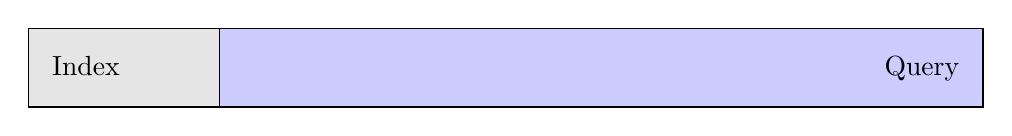
\begin{tikzpicture}
        \node (bar) at(0,0) [
            rectangle, anchor=west,
            minimum width=\columnwidth, minimum height=1cm,
            draw=black, thin,
            fill=gray!20,
        ] {};

        \node at(bar.east) [
            rectangle, anchor=east,
            minimum width=0.8\columnwidth, minimum height=1cm,
            draw=black, thin,
            fill=blue!20,
        ] {};

        \node at(bar.west) [
            rectangle, anchor=west, inner xsep=2ex,
            text height=1.5ex, text depth=0.25ex,
            text=black,
        ] {Index};
        \node at(bar.east) [
            rectangle, anchor=east, inner xsep=2ex,
            text height=1.5ex, text depth=0.25ex,
            text=black,
        ] {Query};
    \end{tikzpicture}

    \begin{center}
        This is an interactive feature, so we can't do too much work at query
        time.
    \end{center}
    \begin{center}
        Goal: < 100ms
    \end{center}
\end{frame}


\begin{frame}[t]
    \frametitle{When do we do the work?}
    \vskip 2em
    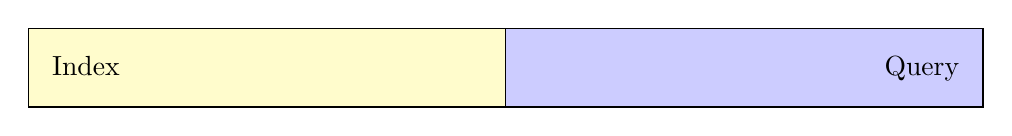
\begin{tikzpicture}
        \node (bar) at(0,0) [
            rectangle, anchor=west,
            minimum width=\columnwidth, minimum height=1cm,
            draw=black, thin,
            fill=gray!20,
        ] {};

        \node at(bar.west) [
            rectangle, anchor=west,
            minimum width=0.5\columnwidth, minimum height=1cm,
            draw=black, thin,
            fill=yellow!20,
        ] {};
        \node at(bar.east) [
            rectangle, anchor=east,
            minimum width=0.5\columnwidth, minimum height=1cm,
            draw=black, thin,
            fill=blue!20,
        ] {};

        \node at(bar.west) [
            rectangle, anchor=west, inner xsep=2ex,
            text height=1.5ex, text depth=0.25ex,
            text=black,
        ] {Index};
        \node at(bar.east) [
            rectangle, anchor=east, inner xsep=2ex,
            text height=1.5ex, text depth=0.25ex,
            text=black,
        ] {Query};
    \end{tikzpicture}

    \begin{center}
        We want to strike a balance.
    \end{center}

    \begin{center}
        Precalculate as much as we can while still being incremental.

        Defer \strong{some} of the work until query time to make that happen.
    \end{center}
\end{frame}


\section{Stack graphs}

\begin{frame}
    \sectionpage
\end{frame}


% incremental_separate_files
\begin{frame}[fragile]
    \frametitle{What would incremental results look like?}

    \uncover<2>{\highlightdef{incremental_separate_files_broil_def}}
    \uncover<3>{\highlightref{incremental_separate_files_broil_ref}}

    \begin{center}
    \begin{minipage}[t]{9em}
    \begin{minted}[autogobble,frame=single,framesep=6pt,label=stove.py,escapeinside=??]{python}
        def bake():
            pass

        def ?\tikzmark{incremental_separate_files_broil_def_start}?broil?\tikzmark{incremental_separate_files_broil_def_end}?():
            pass

        def saute():
            pass
    \end{minted}
    \end{minipage}
    \hspace{0.5em}
    \begin{minipage}[t]{11em}
    \begin{minted}[autogobble,frame=single,framesep=6pt,label=kitchen.py,escapeinside=??]{python}
        from stove import ?\tikzmark{incremental_separate_files_broil_import}?broil

        ?\tikzmark{incremental_separate_files_broil_ref_start}?broil?\tikzmark{incremental_separate_files_broil_ref_end}?()
    \end{minted}
    \end{minipage}
    \end{center}

    \begin{overprint}
        \onslide<2>\centerline{\texttt{stove.broil} is defined at \textsl{stove.py:4:4}}
        \onslide<3>\centerline{The reference at \textsl{kitchen.py:3:1} might refer to \texttt{stove.broil}}
    \end{overprint}
\end{frame}


\begin{frame}
    \begin{center}
        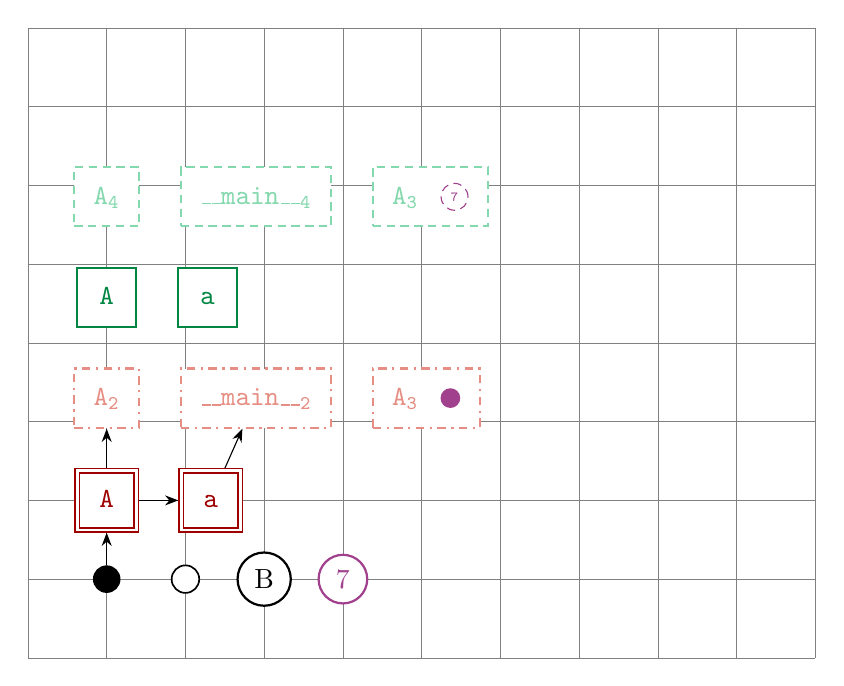
\begin{tikzpicture}
            \draw [help lines] (0,0) grid (10,8);

            \node (root)   [root node]       at(1,1)  {};
            \node (s0)     [anon scope]      at(2,1)  {};
            \node (sB)     [named scope]     at(3,1)  {B};
            \node (s7)     [exported scope]  at(4,1)  {7};
            \node (A)      [definition]      at(1,2)  {A};

            \node (a)      [definition]  [right=of A] {a};
            \node (A2)     [pop]         [above=of A] {A\textsubscript{2}};
            \node (main2)  [pop]         [right=of A2] {\_\_main\_\_\textsubscript{2}};
            \node (bar)    [pop]         [right=of main2] {A\textsubscript{3} \popscope};

            \node (A3)     [reference]  [above=of A2] {A};
            \node (a3)     [reference]  [right=of A3] {a};
            \node (A4)     [push]       [above=of A3] {A\textsubscript{4}};
            \node (main4)  [push]       [right=of A4] {\_\_main\_\_\textsubscript{4}};
            \node (foo)    [push]       [right=of main4] {A\textsubscript{3} \pushscope{7}};

            % edges
            \path [-Stealth]
              (root) edge (A)
              (A) edge (a)
                  edge (A2)
              (a) edge (main2)
              ;
        \end{tikzpicture}
    \end{center}
\end{frame}

\begin{frame}[fragile]
    \begin{columns}
    \begin{column}{0.3\textwidth}
        \begin{minted}[autogobble,frame=single,framesep=6pt,label=a.py,escapeinside=??]{python}
            def broil?\tikzmark{testbroildef}?():
                pass

            def fry():
                pass

            broil?\tikzmark{testbroilref}?()
        \end{minted}
        \uncover<1>  {\curvecodeline{[yshift=8pt] pic cs:testbroilref}{+(25:2cm) and +(-45:1cm)}{[yshift=-4pt] pic cs:testbroildef}} \uncover<2- >{\codeline{pic cs:testbroilref}{pic cs:testbroildef}}
    \end{column}

    \begin{column}{0.7\textwidth}
        \begin{center}
        \begin{tikzpicture}
            \node (root)       [root node]                            {};
            \node (a)          [definition]  [right=of root]          {a};
            \node (dot)        [pop]         [right=of a]             {.};
            \node (s1)         [anon scope]  [right=of dot]           {};

            \setwidestsymbol{broil}
            \node (s2)         [anon scope]  [above=\scopegap of s1]  {};
            \node (broil ref)  [reference]   [right=of s2]            {\sized{broil}};
            \node (s3)         [anon scope]  [above=\scopegap of s2]  {};
            \node (fry)        [definition]  [right=of s3]  [highlight node on=<1->] {\sized{fry}};
            \node (s4)         [anon scope]  [above=\scopegap of s3]  {};
            \node (broil def)  [definition]  [right=of s4]            {\sized{broil}};
            \node (s5)         [anon scope]  [above=\scopegap of s4]  {};

            \path [-Stealth]
              (root)      edge (a)
              (a)         edge (dot)
              (dot)       edge (s1)
              (s1)        edge (s2)
              (broil ref) edge [show path on=<2>] (s2)
              (s2)        edge [show path on=<3>] (s3)
              (s3)        edge (s4)
                          edge (fry)
              (s4)        edge (s5)
                          edge (broil def)
              ;
        \end{tikzpicture}
        \end{center}
    \end{column}
    \end{columns}
\end{frame}

\end{document}
